\documentclass[a4paper]{report}

\usepackage{cmap} % Улучшенный поиск русских слов в полученном pdf-файле
\usepackage[T2A]{fontenc} % Поддержка русских букв
\usepackage[utf8]{inputenc} % Кодировка utf8
\usepackage[english,russian]{babel} % Языки: русский, английский

% \usepackage{setspace}
% \onehalfspacing % Полуторный интервал

\frenchspacing
\usepackage{indentfirst} % Красная строка

%                30                    20           20
\usepackage[left=20mm, right=10mm, top=15mm, bottom=15mm]{geometry}

\usepackage{titlesec}
\titlespacing*{\chapter}{0pt}{-30pt}{8pt}
\titlespacing*{\section}{\parindent}{*4}{*4}
\titlespacing*{\subsection}{\parindent}{*4}{*4}
\titleformat{\chapter}{\LARGE\bfseries}{\thechapter}{20pt}{\LARGE\bfseries}
\titleformat{\section}{\Large\bfseries}{\thesection}{20pt}{\Large\bfseries}

\usepackage{amsmath}
\usepackage{amssymb}
\usepackage{commath}
\usepackage{icomma}

\usepackage[unicode,pdftex]{hyperref} % Ссылки в pdf
\hypersetup{hidelinks}

\usepackage{graphicx}

%% begin theorem
\usepackage{amsthm}

\makeatletter
\newtheoremstyle{indented}
	{}% measure of space to leave above the theorem
	{}% measure of space to leave below the theorem
	{}% name of font to use in the body of the theorem
	{\parindent}% measure of space to indent
	{\bfseries}% name of head font
	{.}% punctuation between head and body
	{ }% space after theorem head; " " = normal interword space
	{}% header specification (empty for default)
\makeatother

\theoremstyle{indented}

\newtheorem{definition}{Определение}[section]
\newtheorem{example}{Пример}[section]
\newtheorem{theorem}{Теорема}[section]
\newtheorem{task}{Задание}

\makeatletter
\DeclareRobustCommand\bfseriesitshape{%
	\not@math@alphabet\itshapebfseries\relax
	\fontseries\bfdefault
	\fontshape\itdefault
	\selectfont
}
\makeatother

\DeclareTextFontCommand{\textbfit}{\bfseriesitshape}
\DeclareTextFontCommand{\define}{\bfseriesitshape}
%% end theorem

%% begin columns
\usepackage{etoolbox,refcount}
\usepackage{multicol}

\newcounter{countitems}
\newcounter{nextitemizecount}
\newcommand{\setupcountitems}{%
	\stepcounter{nextitemizecount}%
	\setcounter{countitems}{0}%
	\preto\item{\stepcounter{countitems}}%
}
\makeatletter
\newcommand{\computecountitems}{%
	\edef\@currentlabel{\number\c@countitems}%
	\label{countitems@\number\numexpr\value{nextitemizecount}-1\relax}%
}
\newcommand{\nextitemizecount}{%
	\getrefnumber{countitems@\number\c@nextitemizecount}%
}
\newcommand{\previtemizecount}{%
	\getrefnumber{countitems@\number\numexpr\value{nextitemizecount}-1\relax}%
}
\makeatother
\newenvironment{AutoMultiColItemize}{%
	\ifnumcomp{\nextitemizecount}{>}{3}{\begin{multicols}{2}}{}%
		\setupcountitems\begin{itemize}}%
		{\end{itemize}%
		\unskip\computecountitems\ifnumcomp{\previtemizecount}{>}{3}{\end{multicols}}{}}
\makeatother
\newenvironment{AutoMultiColEnumerate}{%
	\ifnumcomp{\nextitemizecount}{>}{3}{\begin{multicols}{2}}{}%
		\setupcountitems\begin{enumerate}}%
		{\end{enumerate}%
		\unskip\computecountitems\ifnumcomp{\previtemizecount}{>}{3}{\end{multicols}}{}}
%% end columns


%% begin code
\usepackage{listings}
\usepackage{xcolor}

\lstdefinestyle{lispinline}{
	language=Lisp,
	backgroundcolor=\color{white},
	basicstyle=\footnotesize\ttfamily,
	keywordstyle=\color{blue},
	stringstyle=\color{red},
	commentstyle=\color{gray},
	tabsize=8,
	captionpos=b,
	breaklines=true,
	breakatwhitespace=true,
	escapeinside={\#*}{*)},
	morecomment=[l][\color{magenta}]{\#}
}

\newcommand{\code}[1]{\texttt{#1}}
%% end code

\usepackage{pgfplots}
\usetikzlibrary{datavisualization}
\usetikzlibrary{datavisualization.formats.functions}


\begin{document}

\begin{titlepage}
	{\large % 14pt instead of 12pt
	\onehalfspacing
	\centering

	\begin{wrapfigure}[7]{l}{0.14\linewidth}
		\vspace{3mm}
		\hspace{-10mm}
		
\includegraphics[width=0.93\linewidth]{inc/img/bmstu-logo}
	\end{wrapfigure}
	{\singlespacing \footnotesize \bfseries Министерство науки и высшего образования Российской Федерации\\Федеральное государственное бюджетное образовательное учреждение\\высшего образования\\<<Московский государственный технический университет\\имени Н.~Э.~Баумана\\ (национальный исследовательский университет)>>\\(МГТУ им. Н.~Э.~Баумана)\\}

	\vspace{-2.2mm}
	\vhrulefill{0.9mm}\\
	\vspace{-7.5mm}
	\vhrulefill{0.2mm}\\
	\vspace{2mm}

	{\doublespacing \small \raggedright ФАКУЛЬТЕТ \hspace{25mm} «Информатика и системы управления»\\
	КАФЕДРА \hspace{5mm} «Программное обеспечение ЭВМ и информационные технологии»\\}

	\vspace{30mm}

	\textbf{ОТЧЁТ}\\
	По лабораторной работе №6\\
	По курсу: «Функциональное и логическое программирование»\\
	%Тема: «Тема работы»\\

	\vspace{60mm}

	\hspace{70mm} Студент:       \hfill Керимов~А.~Ш.\\
	\hspace{70mm} Группа:        \hfill ИУ7-64Б\\
	\hspace{70mm} Преподаватели: \hfill Толпинская~Н.~Б.,\\
	                             \hfill Строганов~Ю.~В.\\

	\vfill

	Москва\\
	\the\year\\}
\end{titlepage}

\setcounter{page}{2}


\begin{task}
	Представить следующие списки в виде списочных ячеек:
	\begin{AutoMultiColEnumerate}
		\item \code{'(open close halph)}
		\item \code{'((open1) (close2) (halph3))}
		\item \code{'((one) for all (and(me(for you))))}
		\item \code{'((TOOL) (call))}
		\item \code{'((TOOL1) ((call2)) ((sell)))}
		\item \code{'(((TOOL) (call)) ((sell)))}
	\end{AutoMultiColEnumerate}
\end{task}

\begin{figure}[!h]
	\begin{tabular}{|l|l|}
		\hline
		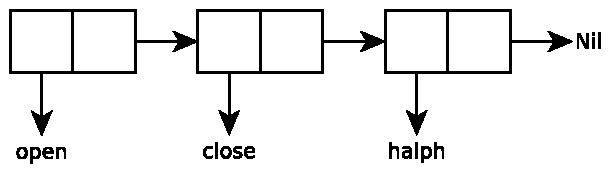
\includegraphics[scale=0.475]{inc/img/task0101.pdf} & 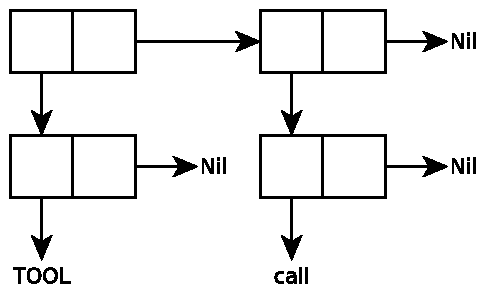
\includegraphics[scale=0.475]{inc/img/task0104.pdf} \\\hline
		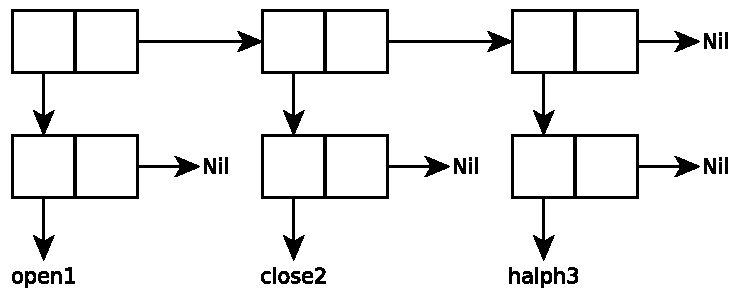
\includegraphics[scale=0.475]{inc/img/task0102.pdf} & 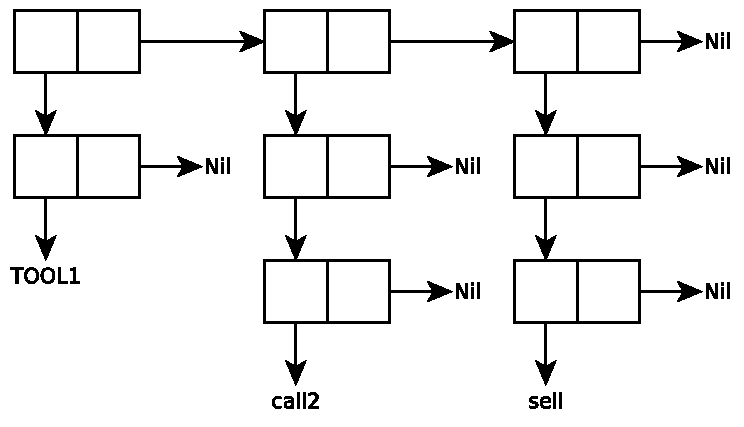
\includegraphics[scale=0.475]{inc/img/task0105.pdf} \\\hline
		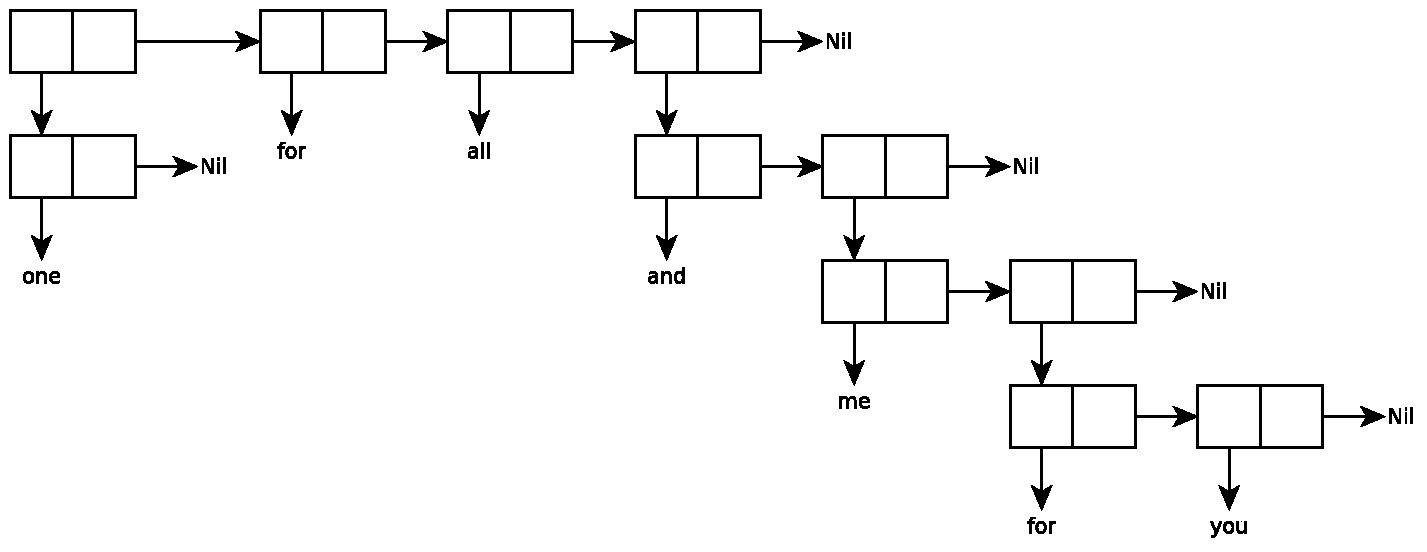
\includegraphics[scale=0.475]{inc/img/task0103.pdf} & 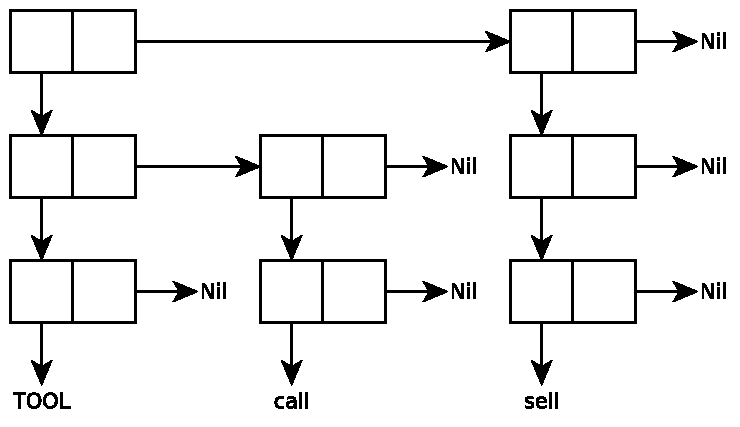
\includegraphics[scale=0.475]{inc/img/task0106.pdf} \\\hline
	\end{tabular}
\end{figure}

\begin{task}
	Используя только функции \code{CAR} и \code{CDR}, написать выражения, возвращающие 1) второй 2) третий 3) четвёртый элементы заданного списка.
\end{task}

\begin{AutoMultiColEnumerate}
	\item
\begin{lstlisting}[style=lispinline]
(car (cdr '(1 2 3 4 5)))             ; second
\end{lstlisting}

	\item
\begin{lstlisting}[style=lispinline]
(car (cdr (cdr '(1 2 3 4 5))))       ; third
\end{lstlisting}

	\item
\begin{lstlisting}[style=lispinline]
(car (cdr (cdr (cdr '(1 2 3 4 5))))) ; fourth
\end{lstlisting}
\end{AutoMultiColEnumerate}

\end{document}
